\documentclass[aspectratio=169,11pt]{beamer}

\usepackage[T1]{fontenc}
\usepackage{lmodern}
\usepackage{amsmath,amssymb,mathtools}
\usepackage{array}
\usepackage{booktabs}
\usepackage{graphicx}
\usepackage{tikz}
\usetikzlibrary{arrows.meta,calc,fit,matrix,positioning}

\definecolor{MSSNavy}{HTML}{12304A}
\definecolor{MSSOrange}{HTML}{D96B1B}
\definecolor{MSSLight}{HTML}{EDF2F5}
\definecolor{MSSGray}{HTML}{617080}
\definecolor{MSSGreen}{HTML}{2E7D63}

\setbeamercolor{normal text}{fg=MSSNavy,bg=white}
\setbeamercolor{frametitle}{fg=MSSNavy,bg=white}
\setbeamercolor{structure}{fg=MSSOrange}
\setbeamercolor{alerted text}{fg=MSSOrange}
\setbeamerfont{frametitle}{size=\LARGE,series=\bfseries}
\setbeamerfont{normal text}{size=\large}
\setbeamerfont{footnote}{size=\tiny}
\setbeamertemplate{navigation symbols}{}
\setbeamertemplate{itemize item}{\color{MSSOrange}\raise0.2ex\hbox{\(\blacktriangleright\)}}
\setbeamersize{text margin left=0.85cm,text margin right=0.85cm}

\newcommand{\source}[1]{%
  \vfill
  {\color{MSSGray}\fontsize{6.5}{7.5}\selectfont #1\par}
}
\newcommand{\orange}[1]{\textcolor{MSSOrange}{#1}}
\newcommand{\navy}[1]{\textcolor{MSSNavy}{#1}}

\input{../generated/unveiling_values.tex}
\input{../generated/figure1_values.tex}
\input{../generated/figure1_authors_values.tex}

\begin{document}

\begin{frame}[plain]
  \begin{tikzpicture}[remember picture,overlay]
    \fill[MSSLight] (current page.south west) rectangle (current page.north east);
    \fill[white,rounded corners=3pt]
      ([xshift=0.65cm,yshift=-0.55cm]current page.north west)
      rectangle
      ([xshift=9.7cm,yshift=-4.9cm]current page.north west);

    % Native schematic: exact equations and data appear in later slides.
    \coordinate (n1) at ([xshift=-5.2cm,yshift=2.15cm]current page.east);
    \coordinate (n2) at ([xshift=-2.8cm,yshift=2.55cm]current page.east);
    \coordinate (n3) at ([xshift=-1.15cm,yshift=0.75cm]current page.east);
    \coordinate (n4) at ([xshift=-3.75cm,yshift=-0.15cm]current page.east);
    \coordinate (n5) at ([xshift=-1.75cm,yshift=-2.05cm]current page.east);
    \coordinate (n6) at ([xshift=-5.0cm,yshift=-2.15cm]current page.east);
    \foreach \a/\b in {n1/n2,n2/n3,n3/n4,n4/n1,n4/n5,n5/n6,n6/n4,n2/n5}
      \draw[MSSNavy,opacity=0.45,line width=1.5pt] (\a) -- (\b);
    \foreach \n in {n1,n3,n5}
      \filldraw[fill=white,draw=MSSOrange,line width=2pt] (\n) circle (0.30cm);
    \foreach \n in {n2,n4,n6}
      \filldraw[fill=white,draw=MSSNavy,line width=2pt] (\n) circle (0.30cm);
    \draw[-{Latex[length=3mm]},MSSOrange,line width=2.4pt]
      (n4) .. controls +(0.7,0.8) and +(-0.7,-0.5) .. (n3);
    \node[anchor=north west,text width=8.35cm,align=left]
      at ([xshift=1.0cm,yshift=-0.9cm]current page.north west) {
      {\fontsize{25}{28}\selectfont\bfseries\color{MSSNavy}
       Unveiling the\\Financial Network}\par
      \vspace{0.25cm}
      {\fontsize{13.5}{16}\selectfont\color{MSSOrange}
       The Leontief core of Mian, Straub, and Sufi (2025)}\par
      \vspace{0.25cm}
      {\fontsize{10}{12}\selectfont\color{MSSGray}
       Sections 2.1--2.2 \(\cdot\) independent course replication}
    };
    \node[anchor=south west,text width=10cm]
      at ([xshift=0.9cm,yshift=0.35cm]current page.south west) {
      {\fontsize{6.5}{7.5}\selectfont\color{MSSGray}
       Native network schematic; it contains no data. Equations follow the
       July 25, 2025 paper.}
    };
  \end{tikzpicture}
\end{frame}

% Include after the scope/version slide in presentation.tex.

\begin{frame}{Replication evidence has three distinct layers}
  \begin{columns}[T,onlytextwidth]
    \column{0.31\textwidth}
    \begin{block}{1. Historical benchmark}
      \small
      Same February 2021 final data, same Stata analysis, same older exhibit.

      \vspace{0.15cm}
      \textbf{Question:} can the supplied package reproduce itself?
    \end{block}

    \column{0.31\textwidth}
    \begin{block}{2. Reconstruction}
      \small
      Earliest feasible author inputs, independently written transformations,
      same economic object.

      \vspace{0.15cm}
      \textbf{Question:} do we understand and rebuild the method?
    \end{block}

    \column{0.31\textwidth}
    \begin{block}{3. New-data robustness}
      \small
      Newer public vintage, harmonized definition, explicitly revised sector
      and sample boundary.

      \vspace{0.15cm}
      \textbf{Question:} does the economic pattern survive updated data?
    \end{block}
  \end{columns}

  \vspace{0.25cm}
  \begin{alertblock}{Evidence rule}
    Robustness is informative, but it does not replace same-input replication.
    Every output must carry both a paper-version and an evidence-layer label.
  \end{alertblock}
  \source{Project evidence hierarchy. The July 2025 paper is the target; the supplied Stata package and final files correspond to February 2021.}
\end{frame}

\begin{frame}{Selective reads keep the full source tree manageable}
  \begin{columns}[T,onlytextwidth]
    \column{0.54\textwidth}
    \begin{block}{The original tree is now available}
      \begin{itemize}
        \item author data tree: about 45 GB apparent
        \item Figure 1 reads only selected FOF, CRSP, and NIPA columns
        \item no duplicate raw tree under \texttt{Data/}
        \item generated annual outputs are only kilobytes
      \end{itemize}
    \end{block}

    \column{0.42\textwidth}
    \begin{block}{Deadline-first sequence}
      \begin{enumerate}
        \item reuse authors' prepared panel
        \item recompute core aggregation
        \item validate annual identities
        \item save compact comparison data
      \end{enumerate}
    \end{block}
  \end{columns}

  \vspace{0.15cm}
  \begin{alertblock}{Protect the vendor snapshot}
    The master script uses \texttt{replace}. Our Python pipeline reads the
    authors' files without mutation and writes only to project-owned outputs.
  \end{alertblock}
  \source{Filesystem metadata audit, 2026-08-08; Figure 1 selective read verified 2026-08-09. Detailed folder map and storage policy: docs/data/author-kit-data-map.md.}
\end{frame}


\begin{frame}{Direct balance sheets stop one layer too early}
  \begin{columns}[T,onlytextwidth]
    \column{0.58\textwidth}
    \centering
    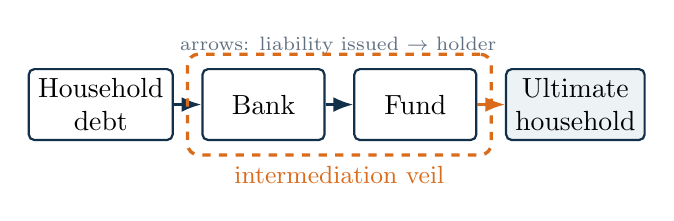
\begin{tikzpicture}[
      node distance=0.35cm,
      entity/.style={draw=MSSNavy,thick,rounded corners=2pt,fill=white,
        minimum width=1.55cm,minimum height=0.9cm,align=center},
      arrow/.style={-{Latex[length=2.5mm]},thick,color=MSSNavy},
      veil/.style={draw=MSSOrange,dashed,very thick,rounded corners=4pt,
        inner sep=5pt}
    ]
      \node[entity] (debt) {Household\\debt};
      \node[entity,right=of debt] (bank) {Bank};
      \node[entity,right=of bank] (fund) {Fund};
      \node[entity,right=of fund,fill=MSSLight] (owner) {Ultimate\\household};
      \draw[arrow] (debt) -- (bank);
      \draw[arrow] (bank) -- (fund);
      \draw[arrow,color=MSSOrange] (fund) -- (owner);
      \node[font=\scriptsize,color=MSSGray] at ($(debt)!0.5!(owner)+(0,0.75)$)
        {arrows: liability issued \(\rightarrow\) holder};
      \node[veil,fit=(bank)(fund),label={[MSSOrange,font=\small]below:intermediation veil}] {};
    \end{tikzpicture}

    \vspace{0.55cm}
    \[
      \text{direct holder} \neq \text{ultimate owner}
    \]

    \column{0.38\textwidth}
    \begin{itemize}
      \item Financial Accounts observe each direct issuer--holder link.
      \item Intermediaries hold claims on one another.
      \item We need the entire chain to ask what household saving ultimately finances.
    \end{itemize}
  \end{columns}
  \source{Source: Mian, Straub, and Sufi (2025), Section 2 and Section 2.1, printed pp. 5--6. Diagram uses the paper's issuer-to-holder orientation.}
\end{frame}

\begin{frame}{Rows issue liabilities; columns hold them}
  \begin{columns}[T,onlytextwidth]
    \column{0.55\textwidth}
    \[
      s_t(i,j)
      =
      \frac{
        \substack{\text{liabilities issued by }i\\
                  \text{and held directly by }j}
      }{
        \text{total liabilities issued by }i
      }
    \]
    \[
      \bar M_t=
      \left[
      \begin{array}{c|c}
        \bar M_t^{OO} & \bar M_t^{OI}\\ \hline
        \bar M_t^{IO} & \bar M_t^{II}
      \end{array}
      \right]
      \quad
      \begin{matrix}
        \left.\vphantom{\bar M_t^{OO}}\right\}\ m\text{ owners}\\[0.45cm]
        \left.\vphantom{\bar M_t^{II}}\right\}\ k\text{ intermediaries}
      \end{matrix}
    \]
    \[
      \bar M_t\mathbf 1=\mathbf 1.
    \]

    \column{0.41\textwidth}
    \begin{block}{Orientation is part of the economics}
      \[
        \textbf{row }i=\text{issuer/borrower}
      \]
      \[
        \textbf{column }j=\text{holder/lender}
      \]
    \end{block}
    \vspace{0.2cm}
    \begin{itemize}
      \item \(m=4\) ultimate owners
      \item \(k=23\) intermediaries
      \item \(27\times27\) matrix of unit-free shares
    \end{itemize}
  \end{columns}
  \source{Source: Mian, Straub, and Sufi (2025), Section 2.1, printed pp. 5--6. \(O\) denotes owners and \(I\) intermediaries.}
\end{frame}

\begin{frame}{A row shows who funds one issuer}
  \begin{columns}[T,onlytextwidth]
    \column{0.48\textwidth}
    \centering
    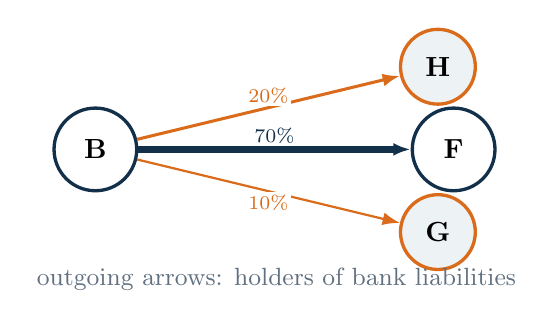
\begin{tikzpicture}[
      x=1cm,y=1cm,
      owner/.style={circle,draw=MSSOrange,very thick,fill=MSSLight,
        minimum size=0.95cm,font=\bfseries},
      intermediary/.style={circle,draw=MSSNavy,very thick,fill=white,
        minimum size=1.05cm,font=\bfseries},
      owneredge/.style={-{Latex[length=2.2mm]},color=MSSOrange,thick},
      crossedge/.style={-{Latex[length=2.2mm]},color=MSSNavy,thick},
      weight/.style={fill=white,inner sep=1pt,font=\scriptsize}
    ]
      \node[intermediary] (b) at (0,0) {B};
      \node[owner] (h) at (4.35,1.05) {H};
      \node[intermediary] (f) at (4.55,0) {F};
      \node[owner] (g) at (4.35,-1.05) {G};

      \draw[owneredge,line width=1.1pt] (b) --
        node[weight,above] {20\%} (h);
      \draw[crossedge,line width=2.5pt] (b) --
        node[weight,above] {70\%} (f);
      \draw[owneredge,line width=0.8pt] (b) --
        node[weight,below] {10\%} (g);

      \node[font=\small,align=center,color=MSSGray] at (2.3,-1.65)
        {outgoing arrows: holders of bank liabilities};
    \end{tikzpicture}
    \vspace{-0.45cm}
    \[
      \sum_j s(B,j)=0.20+0.70+0.10=1.
    \]

    \column{0.48\textwidth}
    {\color{MSSOrange}\bfseries Outgoing from B: funding mix}

    B issues liabilities held by H, F, and G. All three shares divide by
    bank liabilities \(L_B\), so the row sums to one.

    \vspace{0.2cm}
    {\color{MSSNavy}\bfseries Incoming to B: a bank asset}

    \(F\longrightarrow B:\ s(F,B)=20\%\). B holds 20\% of
    \emph{the fund's liabilities}. The denominator is \(L_F\), so this is not
    20\% of bank lending.

    \vspace{0.12cm}
    {\small Intermediaries own assets directly, but are not terminal owners.}

    \vspace{0.12cm}
    Thus \(\bar M\mathbf 1=\mathbf 1\); columns have no unit-sum restriction.
  \end{columns}
  \source{Source: Mian, Straub, and Sufi (2025), Section 2.1, printed pp. 5--6. Values come from the generated four-sector example. ``Funded by'' includes all liability instruments, not only literal bank loans.}
\end{frame}

\begin{frame}{Equation (4) turns dollar holdings into ownership shares}
  \[
    \boxed{
    \bar M_t
    =
    \left(\frac{1}{L_t}\right)^{\!\top}
    \odot
    \left(\sum_{h=1}^{\ell}M_{h,t}\right),
    \qquad \ell=34
    }
  \]
  \vspace{0.2cm}
  \begin{center}
  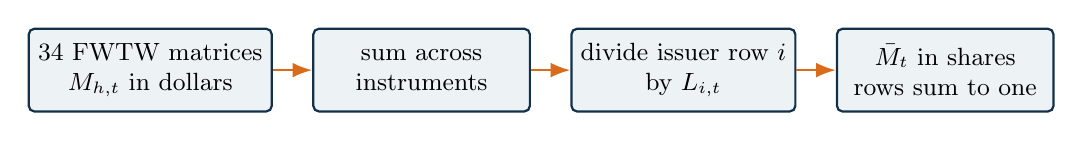
\begin{tikzpicture}[
    box/.style={draw=MSSNavy,thick,rounded corners=2pt,fill=MSSLight,
      minimum width=2.75cm,minimum height=1.05cm,align=center,font=\small},
    arrow/.style={-{Latex[length=2.5mm]},thick,color=MSSOrange}
  ]
    \node[box] (instruments) {34 FWTW matrices\\\(M_{h,t}\) in dollars};
    \node[box,right=0.5cm of instruments] (sum) {sum across\\instruments};
    \node[box,right=0.5cm of sum] (scale) {divide issuer row \(i\)\\by \(L_{i,t}\)};
    \node[box,right=0.5cm of scale] (shares) {\(\bar M_t\) in shares\\rows sum to one};
    \draw[arrow] (instruments) -- (sum);
    \draw[arrow] (sum) -- (scale);
    \draw[arrow] (scale) -- (shares);
  \end{tikzpicture}
  \end{center}
  \vspace{0.2cm}
  \begin{alertblock}{Current input boundary}
    Estimating unknown FWTW cells is upstream. Our constructor accepts completed
    instrument matrices and fails if the resulting rows do not sum to one.
  \end{alertblock}
  \source{Source: Mian, Straub, and Sufi (2025), Section 2.2, printed pp. 8--9, Equation (4). FWTW means from-where-to-where.}
\end{frame}

\begin{frame}{Missing cells are completed within each instrument}
  \fontsize{8.9}{10.6}\selectfont
  For instrument \(h\), \(X_{h,t}(i,j)\) is a \emph{dollar stock}: liabilities
  issued by sector \(i\) and held by sector \(j\).
  \begin{columns}[T,onlytextwidth]
    \column{0.52\textwidth}
    \[
      \begin{array}{c|ccc|c}
        & H & B & F & \text{issuance total}\\ \hline
        i_1 & x & ? & x & r_{1ht}\\
        i_2 & ? & x & ? & r_{2ht}\\
        i_3 & x & x & ? & r_{3ht}\\ \hline
        \text{holding total} & c_{Hht} & c_{Bht} & c_{Fht} & T_{ht}
      \end{array}
    \]
    \[
      r_{iht}=\sum_jX_{h,t}(i,j),\qquad
      c_{jht}=\sum_iX_{h,t}(i,j).
    \]

    \column{0.44\textwidth}
    \begin{block}{How the question marks are filled}
      \begin{itemize}
        \item use exact bilateral positions when observed;
        \item one unknown against a known margin is an arithmetic residual;
        \item several unknowns are not uniquely identified: use exclusion,
          proportionality, and row--column balancing rules.
      \end{itemize}
    \end{block}
    \begin{alertblock}{DINA is not part of this completion}
      These constraints come from Financial Accounts totals and detailed FWTW
      information, separately for each instrument.
    \end{alertblock}
  \end{columns}
  \vspace{0.05cm}
  \centering
  \orange{34 instrument matrices} \(\longrightarrow\) \navy{one network over 23 intermediary sectors and 4 owners}
  \source{Source: MSS (2025), Section 2.2, printed pp. 8--9. Batty et al. completion uses known cells, proportionality, and consistency with instrument-specific row and column totals. Symbols \(x\) and \(?\) are schematic.}
\end{frame}

\begin{frame}{DINA splits the household column; it does not build the network}
  \fontsize{8.8}{10.5}\selectfont
  Let \(a(h)\) map Financial Accounts instrument \(h\) to a DINA wealth class,
  and let \(\omega_{g,t}^{a}\) be cohort \(g\)'s share of household wealth class
  \(a\). Operationally, the household position is split as
  \[
    \boxed{
      X^{\mathrm{aug}}_{h,t}(i,g)
      =X_{h,t}(i,H)\,\omega_{g,t}^{a(h)},
      \qquad \sum_g\omega_{g,t}^{a}=1
    }.
  \]
  \begin{columns}[T,onlytextwidth]
    \column{0.58\textwidth}
    \centering
    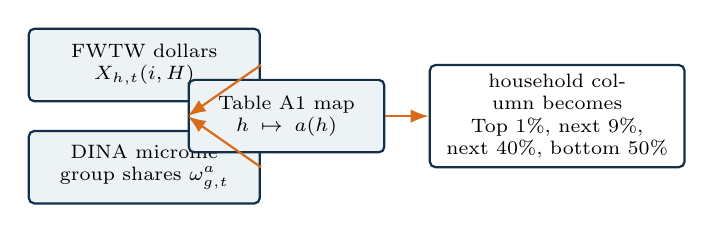
\begin{tikzpicture}[
      box/.style={draw=MSSNavy,thick,rounded corners=2pt,fill=MSSLight,
        minimum height=0.92cm,align=center,font=\scriptsize},
      arrow/.style={-{Latex[length=2.3mm]},thick,color=MSSOrange}
    ]
      \node[box,text width=2.7cm] (fa) {FWTW dollars\\\(X_{h,t}(i,H)\)};
      \node[box,text width=2.7cm,below=0.35cm of fa] (dina)
        {DINA microfile\\group shares \(\omega_{g,t}^{a}\)};
      \node[box,text width=2.25cm,right=0.55cm of $(fa)!0.5!(dina)$] (map)
        {Table A1 map\\\(h\mapsto a(h)\)};
      \node[box,text width=3.0cm,right=0.55cm of map,fill=white] (aug)
        {household column becomes\\Top 1\%, next 9\%, next 40\%, bottom 50\%};
      \draw[arrow] (fa.east) -- (map.west);
      \draw[arrow] (dina.east) -- (map.west);
      \draw[arrow] (map) -- (aug);
    \end{tikzpicture}

    \column{0.38\textwidth}
    \begin{block}{What DINA contributes}
      Tax-record-based microfiles impute wealth by broad asset class, then are
      collapsed to cohort shares.
    \end{block}
    \begin{alertblock}{What DINA does not observe}
      It is not a complete
      \((\text{group},\text{issuer},\text{instrument})\) counterparty table.
    \end{alertblock}
  \end{columns}
  Rebuild \(\bar M_t^{\mathrm{aug}}\), repeat Equation (1), and the unveiled
  primary-asset matrix can be read by wealth cohort.
  \source{Source: MSS (2025), Sections 3.1 and 4.1, printed pp. 15 and 26--27; Appendix Table A1 maps Financial Accounts instruments to DINA and DFA asset classes. The displayed split makes the paper's stated mapping operational.}
\end{frame}

\begin{frame}{Matrix powers add one intermediation layer at a time}
  \begin{columns}[T,onlytextwidth]
    \column{0.46\textwidth}
    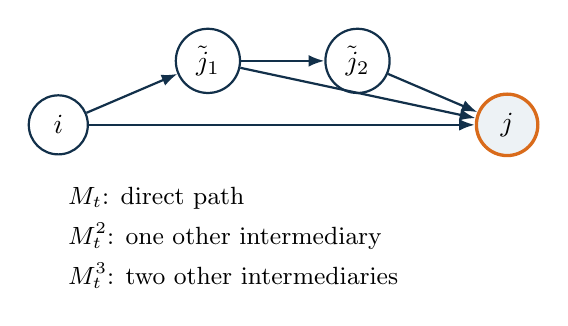
\begin{tikzpicture}[
      x=1.9cm,y=1.25cm,
      node/.style={circle,draw=MSSNavy,thick,minimum size=0.75cm,fill=white},
      owner/.style={circle,draw=MSSOrange,very thick,minimum size=0.78cm,fill=MSSLight},
      arrow/.style={-{Latex[length=2mm]},thick,color=MSSNavy}
    ]
      \node[node] (i) at (0,0) {\(i\)};
      \node[node] (a) at (1,0.65) {\(\tilde j_1\)};
      \node[node] (b) at (2,0.65) {\(\tilde j_2\)};
      \node[owner] (j) at (3,0) {\(j\)};
      \draw[arrow] (i) -- (j);
      \draw[arrow] (i) -- (a);
      \draw[arrow] (a) -- (j);
      \draw[arrow] (a) -- (b);
      \draw[arrow] (b) -- (j);
      \node[align=left,font=\small,anchor=west] at (0,-1.15) {
        \(M_t\): direct path\\[0.12cm]
        \(M_t^2\): one other intermediary\\[0.12cm]
        \(M_t^3\): two other intermediaries
      };
    \end{tikzpicture}

    \column{0.50\textwidth}
    Set the first \(m\) \emph{rows} of \(\bar M_t\) to zero:
    \[
      M_t=
      \begin{bmatrix}
        0&0\\
        B_t&Q_t
      \end{bmatrix}.
    \]
    This stops a path when it reaches an owner while preserving the owner
    columns that receive the claim.
    \[
      (M_t^2)_{ij}
      =
      \sum_{\tilde j=m+1}^{m+k}
      s_t(i,\tilde j)s_t(\tilde j,j).
    \]
  \end{columns}
  \source{Source: Mian, Straub, and Sufi (2025), Section 2.1, printed pp. 6--7. \(B_t\): owner holdings; \(Q_t\): cross-holdings.}
\end{frame}

\begin{frame}{The Leontief solve sums arbitrarily long chains}
  \[
    \bar\Omega_t
    \equiv
    M_t+M_t^2+M_t^3+\cdots
    =
    M_t(I-M_t)^{-1}.
    \tag{1}
  \]
  \begin{columns}[T,onlytextwidth]
    \column{0.52\textwidth}
    The lower-left \(k\times m\) block is
    \[
      \boxed{
      \Omega_t=(I_k-Q_t)^{-1}B_t
      }
    \]
    \[
      (I_k-Q_t)\Omega_t=B_t.
    \]

    \column{0.44\textwidth}
    \begin{block}{Economic condition}
      \[
        \rho(Q_t)<1
      \]
      Cross-holdings eventually resolve to ultimate owners.
    \end{block}
    \begin{block}{Implementation}
      \ttfamily\small
      np.linalg.solve(\\
      \quad I - Q, B\\
      )
    \end{block}
  \end{columns}
  \source{Source: Mian, Straub, and Sufi (2025), Section 2.1, printed p. 7, Equation (1). The block solve is algebraically equivalent and avoids an explicit numerical inverse.}
\end{frame}

\begin{frame}{Each matrix entry is one directed ownership edge}
  \begin{columns}[T,onlytextwidth]
    \column{0.43\textwidth}
    \centering
    \small Sector order: \(H,G,B,F\)
    \[
      \bar M=
      \begin{bmatrix}
        \ToyDirectOwnershipBody
      \end{bmatrix}
    \]
    \vspace{-0.15cm}
    \begin{align*}
      B&=\begin{bmatrix}\ToyBBody\end{bmatrix}, &
      Q&=\begin{bmatrix}\ToyQBody\end{bmatrix}.
    \end{align*}
    \begin{minipage}{0.94\linewidth}
      \small
      \textcolor{MSSOrange}{Orange}: direct claims on owners, \(B\).\\
      \textcolor{MSSNavy}{Navy}: intermediary cross-holdings, \(Q\).
    \end{minipage}

    \column{0.53\textwidth}
    \centering
    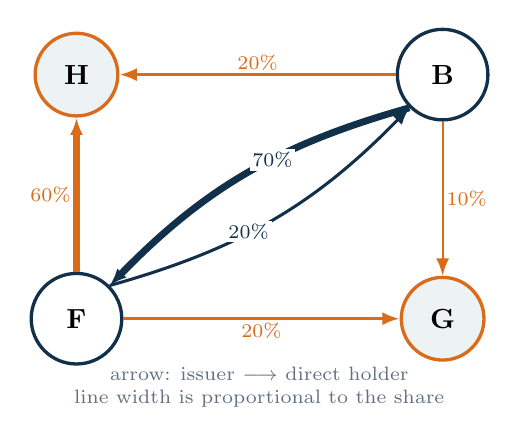
\begin{tikzpicture}[
      x=1cm,y=1cm,
      owner/.style={circle,draw=MSSOrange,very thick,fill=MSSLight,
        minimum size=1.05cm,font=\bfseries},
      intermediary/.style={circle,draw=MSSNavy,very thick,fill=white,
        minimum size=1.15cm,font=\bfseries},
      owneredge/.style={-{Latex[length=2.2mm]},color=MSSOrange,thick},
      crossedge/.style={-{Latex[length=2.2mm]},color=MSSNavy,thick},
      weight/.style={fill=white,inner sep=1pt,font=\scriptsize}
    ]
      \node[owner] (h) at (0,1.55) {H};
      \node[owner] (g) at (4.65,-1.55) {G};
      \node[intermediary] (b) at (4.65,1.55) {B};
      \node[intermediary] (f) at (0,-1.55) {F};

      \draw[owneredge,line width=1.1pt] (b) --
        node[weight,above] {20\%} (h);
      \draw[owneredge,line width=0.8pt] (b) --
        node[weight,right] {10\%} (g);
      \draw[owneredge,line width=2.2pt] (f) --
        node[weight,left] {60\%} (h);
      \draw[owneredge,line width=1.1pt] (f) --
        node[weight,below] {20\%} (g);

      \draw[crossedge,line width=2.5pt] (b.south west)
        to[bend right=15] node[weight,above right] {70\%} (f.north east);
      \draw[crossedge,line width=1.1pt] (f.north east)
        to[bend right=15] node[weight,below left] {20\%} (b.south west);

      \node[font=\scriptsize,color=MSSGray,align=center] at (2.32,-2.42)
        {arrow: issuer \(\longrightarrow\) direct holder\\
         line width is proportional to the share};
    \end{tikzpicture}
  \end{columns}
  \source{All shares are generated from Code/examples/leontief\_unveiling.py via Code/scripts/build\_unveiling\_teaching\_assets.py. Owner self-holdings in the first two rows are stopping states and are not redrawn. Illustrative values, not empirical estimates.}
\end{frame}

\begin{frame}{The fund raises bank household ownership to 72.09\%}
  \begin{columns}[T,onlytextwidth]
    \column{0.57\textwidth}
    \small
    \setlength{\jot}{2pt}
    Let \(\omega_{BH}\) and \(\omega_{FH}\) denote ultimate household shares.
    The network itself gives the fixed point:
    \begin{align*}
      \omega_{BH}&=0.20+0.70\,\omega_{FH},\\
      \omega_{FH}&=0.60+0.20\,\omega_{BH}.
    \end{align*}
    Substitution makes the reciprocal loop explicit:
    \[
      \omega_{BH}=0.62+0.14\,\omega_{BH}
      \quad\Longrightarrow\quad
      \boxed{\omega_{BH}=0.72093}.
    \]
    \vspace{-0.1cm}
    \[
      \underbrace{\ToyBankDirectHousehold}_{\text{direct}}
      +
      \underbrace{70\%\times\ToyFundUltimateHousehold}_{
        \text{through fund }=\ToyBankViaFundHousehold}
      =\underbrace{\ToyBankUltimateHousehold}_{\text{ultimate}}.
    \]
    \vspace{-0.15cm}
    {\scriptsize Path expansion:
      \(\ToyBankHouseholdPathPreview=\ToyBankUltimateHousehold\).}

    \column{0.39\textwidth}
    \centering
    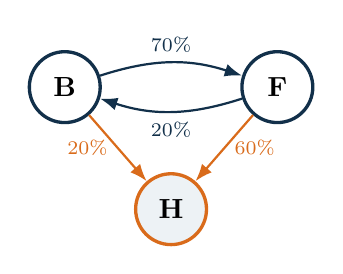
\begin{tikzpicture}[
      intermediary/.style={circle,draw=MSSNavy,very thick,fill=white,
        minimum size=0.9cm,font=\bfseries},
      owner/.style={circle,draw=MSSOrange,very thick,fill=MSSLight,
        minimum size=0.9cm,font=\bfseries},
      edge/.style={-{Latex[length=2.2mm]},thick,color=MSSNavy},
      owneredge/.style={-{Latex[length=2.2mm]},thick,color=MSSOrange}
    ]
      \node[intermediary] (b) at (0,0) {B};
      \node[intermediary] (f) at (2.7,0) {F};
      \node[owner] (h) at (1.35,-1.55) {H};
      \draw[edge] (b) to[bend left=18] node[above,font=\scriptsize] {70\%} (f);
      \draw[edge] (f) to[bend left=18] node[below,font=\scriptsize] {20\%} (b);
      \draw[owneredge] (b) -- node[left,font=\scriptsize] {20\%} (h);
      \draw[owneredge] (f) -- node[right,font=\scriptsize] {60\%} (h);
    \end{tikzpicture}
    \vspace{-0.15cm}

    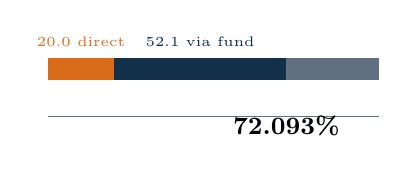
\begin{tikzpicture}[x=0.042cm,y=0.55cm]
      \draw[MSSGray,thin] (0,0) -- (100,0);
      \draw[MSSOrange,line width=8pt] (0,1.1) -- (20,1.1);
      \draw[MSSNavy,line width=8pt] (20,1.1) -- (72.093,1.1);
      \draw[MSSGray,line width=8pt] (72.093,1.1) -- (100,1.1);
      \node[anchor=south,font=\tiny,color=MSSOrange] at (10,1.4)
        {20.0 direct};
      \node[anchor=south,font=\tiny,color=MSSNavy] at (46,1.4)
        {52.1 via fund};
      \node[anchor=north,font=\bfseries\small] at (72.093,0.25)
        {72.093\%};
    \end{tikzpicture}
    \vspace{-0.12cm}
    \[
      \Omega=
      \begin{bmatrix}\ToyOmegaBody\end{bmatrix}.
    \]
  \end{columns}
  \source{Numbers generated by Code/scripts/build\_unveiling\_teaching\_assets.py and verified by the fixed-point test. The illustration is conceptual and contains no data; exact weights are the LaTeX network and equations.}
\end{frame}

\begin{frame}{Equation (2) reconnects ownership to balance sheets}
  \[
    \boxed{
      W_t=L_t\bar M_t-L_t
    }
    \tag{2}
  \]
  \begin{columns}[T,onlytextwidth]
    \column{0.49\textwidth}
    \begin{block}{Assets}
      \(L_t\bar M_t\) allocates the dollar liabilities issued by every sector
      to the sectors that hold them as assets.
    \end{block}

    \column{0.47\textwidth}
    \begin{block}{Minus own liabilities}
      Subtracting \(L_t\) produces each sector's net worth \(W_t\), measured
      in dollars.
    \end{block}
  \end{columns}
  \vspace{0.3cm}
  \[
    \underbrace{\sum_{i=1}^{m+k}W_{i,t}}_{\text{closed-system net worth}}
    =
    0.
  \]
  \source{Source: Mian, Straub, and Sufi (2025), Section 2.1, printed p. 7, Equation (2). The zero-sum identity follows from the row sums of \(\bar M_t\).}
\end{frame}

\begin{frame}{Equation (3) reveals the real uses financed behind intermediaries}
  \[
    \boxed{
      \underset{n\times m}{A_t}
      =
      \underset{n\times k}{P_t}
      \underset{k\times m}{\Omega_t}
      +
      \underset{n\times m}{\Lambda_t}
    }
    \tag{3}
  \]
  \begin{columns}[T,onlytextwidth]
    \column{0.48\textwidth}
    \begin{itemize}
      \item \(P_t\): primary assets held directly by intermediaries
      \item \(\Lambda_t\): primary assets held directly by owners
      \item \(A_t\): final owner shares, direct plus unveiled
    \end{itemize}

    \column{0.48\textwidth}
    \begin{block}{Eight primary assets}
      Household debt; federal debt; state/local debt; foreign credit; real
      estate; corporate business; non-corporate business; residual.
    \end{block}
    \[
      A_t\mathbf 1_m=\mathbf 1_n.
    \]
  \end{columns}
  \source{Source: Mian, Straub, and Sufi (2025), Section 2.1, printed pp. 7--8, Equation (3). All matrices on this slide contain ownership shares.}
\end{frame}

\begin{frame}{The Python core mirrors the paper in six readable lines}
  \begin{columns}[T,onlytextwidth]
    \column{0.58\textwidth}
    \begin{block}{\texttt{unveiled\_ownership()}}
    \ttfamily\fontsize{9.5}{12}\selectfont
    B = direct[n\_owners:, :n\_owners]\\[0.1cm]
    Q = direct[n\_owners:, n\_owners:]\\[0.1cm]
    identity = np.eye(n\_intermediaries)\\[0.25cm]
    return np.linalg.solve(identity - Q, B)
    \end{block}

    \column{0.38\textwidth}
    \begin{block}{Validate once at entry}
      \begin{itemize}
        \item square, finite, non-negative
        \item rows of \(\bar M_t\) sum to one
        \item \(\rho(Q_t)<1\)
      \end{itemize}
    \end{block}
    \begin{block}{Verify economically}
      \begin{itemize}
        \item rows of \(\Omega_t\) sum to one
        \item \(\sum_iW_{i,t}=0\)
        \item closed form equals round sum
      \end{itemize}
    \end{block}
  \end{columns}
  \source{Implementation: Code/unveiling/network.py. Tests: Code/tests/test\_network.py. The block solve is Equation (1a) in docs/methods/leontief-unveiling.md.}
\end{frame}

\begin{frame}{The 2021 kit unveils debt through seven explicit rounds}
  \begin{center}
  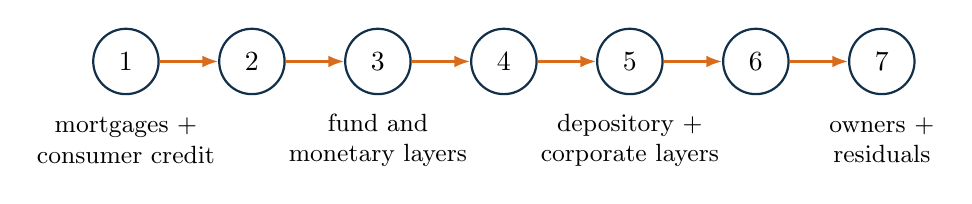
\begin{tikzpicture}[
    round/.style={draw=MSSNavy,thick,circle,minimum size=0.83cm,fill=white},
    arrow/.style={-{Latex[length=2mm]},thick,color=MSSOrange}
  ]
    \foreach \x/\label in {0/1,1.6/2,3.2/3,4.8/4,6.4/5,8.0/6,9.6/7}
      \node[round] (r\label) at (\x,0) {\label};
    \foreach \a/\b in {1/2,2/3,3/4,4/5,5/6,6/7}
      \draw[arrow] (r\a) -- (r\b);
    \node[font=\small,align=center] at (0,-1.0) {mortgages +\\consumer credit};
    \node[font=\small,align=center] at (3.2,-1.0) {fund and\\monetary layers};
    \node[font=\small,align=center] at (6.4,-1.0) {depository +\\corporate layers};
    \node[font=\small,align=center] at (9.6,-1.0) {owners +\\residuals};
  \end{tikzpicture}
  \end{center}
  \begin{columns}[T,onlytextwidth]
    \column{0.48\textwidth}
    \begin{block}{Three parallel pipelines}
      Household debt, government debt, and mortgage debt are unveiled
      separately, then merged into \texttt{Yunveil.dta}.
    \end{block}
    \column{0.48\textwidth}
    \begin{block}{Conservation in Stata}
      \ttfamily\small
      egen test7 = rowtotal(a\_*\_hhd7)\\
      tsline test7 test6
    \end{block}
  \end{columns}
  \source{Source: MSS2021Febreplicationkit/code/build\_fa\_unveiling\_data.do, household-debt rounds at lines 131, 724, 1066, 1259, 1740, 2138, and 2316; final aggregation at 2385--2405.}
\end{frame}

\begin{frame}{Same recursion, different implementation}
  \centering
  \fontsize{8.6}{10.2}\selectfont
  \begin{tabular}{@{}>{\raggedright\arraybackslash}p{2.35cm}
    >{\raggedright\arraybackslash}p{5.35cm}
    >{\raggedright\arraybackslash}p{5.35cm}@{}}
    \toprule
    & \textbf{2025 paper + our Python} & \textbf{February 2021 Stata kit}\\
    \midrule
    Representation
      & One \(27\times27\) direct ownership matrix
      & Instrument- and sector-specific dollar variables\\[0.08cm]
    Unwinding
      & Infinite path sum via a linear solve
      & Seven named reallocation rounds\\[0.08cm]
    Scope
      & Full network, then eight primary assets
      & Three debt categories handled separately\\[0.08cm]
    Adjustments
      & Completed FWTW cells upstream
      & Proportionality, net issuance, and residuals\\[0.08cm]
    Check
      & Owner rows sum to one; \(\rho(Q)<1\)
      & \texttt{test1}--\texttt{test7} conserve debt totals\\
    \bottomrule
  \end{tabular}
  \vspace{0.18cm}

  \begin{alertblock}{Verdict}
    \fontsize{8.6}{10.2}\selectfont
    The economic logic is the same: recursively attribute intermediary assets
    according to liability ownership. Numerical identity is not yet testable:
    the old code is not a fixed-matrix truncation, and the 2025 completed
    matrices are absent from the kit.
  \end{alertblock}
  \source{Sources: Mian, Straub, and Sufi (2025), Sections 2.1--2.2; MSS2021Febreplicationkit/code/build\_fa\_unveiling\_data.do; project crosswalk in docs/methods/leontief-unveiling.md.}
\end{frame}

\begin{frame}{Each main figure consumes a different data layer}
  \fontsize{8.3}{9.8}\selectfont
  \centering
  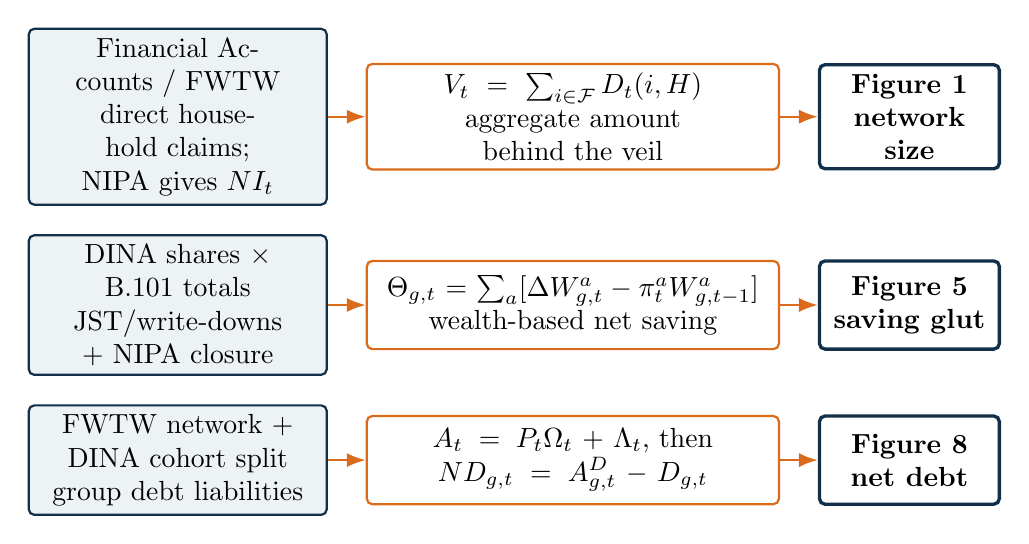
\begin{tikzpicture}[
    sourcebox/.style={draw=MSSNavy,thick,rounded corners=2pt,fill=MSSLight,
      text width=3.55cm,minimum height=1.12cm,align=center},
    objectbox/.style={draw=MSSOrange,thick,rounded corners=2pt,fill=white,
      text width=5.0cm,minimum height=1.12cm,align=center},
    resultbox/.style={draw=MSSNavy,very thick,rounded corners=2pt,fill=white,
      text width=2.05cm,minimum height=1.12cm,align=center,font=\bfseries},
    arrow/.style={-{Latex[length=2.4mm]},thick,color=MSSOrange},
    node distance=0.36cm and 0.48cm
  ]
    \node[sourcebox] (fa1) {Financial Accounts / FWTW\\direct household claims; NIPA gives \(NI_t\)};
    \node[objectbox,right=of fa1] (obj1) {\(V_t=\sum_{i\in\mathcal F}D_t(i,H)\)\\aggregate amount behind the veil};
    \node[resultbox,right=of obj1] (fig1) {Figure 1\\network size};

    \node[sourcebox,below=of fa1] (save) {DINA shares \(\times\) B.101 totals\\JST/write-downs + NIPA closure};
    \node[objectbox,right=of save] (obj5) {\(\Theta_{g,t}=\sum_a[\Delta W^a_{g,t}-\pi^a_tW^a_{g,t-1}]\)\\wealth-based net saving};
    \node[resultbox,right=of obj5] (fig5) {Figure 5\\saving glut};

    \node[sourcebox,below=of save] (debt) {FWTW network + DINA cohort split\\group debt liabilities};
    \node[objectbox,right=of debt] (obj8) {\(A_t=P_t\Omega_t+\Lambda_t\), then\\\(ND_{g,t}=A^D_{g,t}-D_{g,t}\)};
    \node[resultbox,right=of obj8] (fig8) {Figure 8\\net debt};

    \draw[arrow] (fa1) -- (obj1); \draw[arrow] (obj1) -- (fig1);
    \draw[arrow] (save) -- (obj5); \draw[arrow] (obj5) -- (fig5);
    \draw[arrow] (debt) -- (obj8); \draw[arrow] (obj8) -- (fig8);
  \end{tikzpicture}
  \vspace{0.22cm}
  \begin{alertblock}{Consumption data are a cross-check, not Figure 5's baseline}
    The 2025 baseline infers saving from wealth changes net of valuation.
    Income less consumption uses DINA income/taxes/transfers plus SCF-based
    consumption shares; CEX and PSID are supporting/alternative evidence and
    are weak at the very top.
  \end{alertblock}
  \source{Source: MSS (2025), Sections 2.3--2.4, 3.1, 3.6, 4.1--4.2, and Appendix C.1. DFA and the 1983--1989 SCF panel are validation sources; Figure numbers refer to the July 2025 paper.}
\end{frame}

\begin{frame}{Figure 1 measures the size of the veil}
  \fontsize{9.4}{11.1}\selectfont
  Let \(D_t(i,H)\) be claims issued by sector \(i\) and held by households,
  in millions of current dollars. For intermediaries \(\mathcal F\),
  \[
    \boxed{V_t=\sum_{i\in\mathcal F}D_t(i,H)}
  \]
  \begin{columns}[T,onlytextwidth]
    \column{0.48\textwidth}
    \begin{block}{Share behind the veil}
      \[
        \frac{V_t}{\sum_{i\ne ROW}D_t(i,H)}
      \]
      Fraction of household U.S. financial assets issued by intermediaries.
    \end{block}

    \column{0.48\textwidth}
    \begin{block}{Scale of the veil}
      \[
        \frac{V_t}{NI_t}
      \]
      Indirectly held stock relative to annual national income.
    \end{block}
  \end{columns}
  \vspace{-0.04cm}
  \begin{alertblock}{Do not subtract the matrices}
    The household directly holds an intermediary claim, but holds its primary
    assets indirectly. Figure 1's object is \(V_t\), not
    \(\Omega_t-\bar M_t\); Equation (1) instead tells us where \(V_t\) goes.
  \end{alertblock}
  \source{Source: Mian, Straub, and Sufi (2025), Section 2.3 and Figure 1, printed pp. 9--10. Authors-data code mapping: Code/unveiling/figure1\_authors.py.}
\end{frame}

\begin{frame}{We reuse preparation, not the economic aggregation}
  \fontsize{8.6}{10.2}\selectfont
  \begin{columns}[T,onlytextwidth]
    \column{0.56\textwidth}
    The paper has \textbf{23 intermediary sectors} and \textbf{34 instruments}:
    these are different dimensions.  The 2021 kit omits the completed FWTW
    matrices, so we reconstruct the available numerator as
    \begin{align*}
      V_t^A={}&C_t+T_t+MMF_t+GSE_t+MF_t+LI_t\\
              &+(PE_t-UPE_t)+FB_t+FE_t.
    \end{align*}
    \begin{block}{Nine retained claim groups}
      Deposits/currency; time deposits; money-market funds; GSE securities;
      mutual funds; life insurance; funded pensions; financial bonds; listed
      financial equity.
    \end{block}

    \column{0.40\textwidth}
    \begin{block}{Authors prepared upstream}
      \begin{itemize}
        \item Z.1 import and wide panel
        \item Q4-ready stock variables
        \item financial-bond issuer split
      \end{itemize}
    \end{block}
    \begin{block}{Recomputed here}
      \begin{itemize}
        \item component sum in dollars
        \item CRSP equity extension
        \item merge to national income
        \item identities and comparison
      \end{itemize}
    \end{block}
  \end{columns}
  \source{Authors' inputs: LQpanel\_2019Q1.dta, Yunveilhhd.dta, CRSP msf.dta, and YinequalityNIPAanalysis.dta. Our implementation: Code/unveiling/figure1\_authors.py. Sample: Q4 stocks, 1963--2016.}
\end{frame}

\begin{frame}{Authors' data closely reproduce the level behind the veil}
  \begin{columns}[T,onlytextwidth]
    \column{0.70\textwidth}
    \centering
    \includegraphics[width=\linewidth,height=5.05cm,keepaspectratio]{../../Results_Proposal/figures/figure1_authors_data_comparison.png}

    \column{0.26\textwidth}
    \fontsize{8.0}{9.4}\selectfont
    {\color{MSSOrange}\normalsize Level, 1963--2016}\par
    MAE: \AuthorFigureLevelMAE\par
    correlation: \AuthorFigureLevelCorrelation\par
    start: \AuthorFigureStartLevel{} vs.
    \PaperDigitizedStartLevel\par
    end: \AuthorFigureEndLevel{} vs.
    \PaperDigitizedEndLevel\par
    \vspace{0.22cm}
    {\color{MSSOrange}\normalsize Share denominator}\par
    broad balance sheet: \AuthorFigureShareBroadMAE{} MAE\par
    old-kit exclusion proxy: \AuthorFigureShareProxyMAE{} MAE\par
    \vspace{0.22cm}
    \textbf{Verdict:} the old-vintage authors-data level match is strong; the exact 2025
    share denominator is not in the kit.
  \end{columns}
  \source{Gray line digitized programmatically from MSS (2025), physical PDF p. 11. Orange/navy use authors' February 2021 inputs plus our documented CRSP financial-equity extension. Values and comparison statistics are generated, not typed.}
\end{frame}

\begin{frame}{Newer FWTW data are robustness evidence, not replication}
  \begin{columns}[T,onlytextwidth]
    \column{0.53\textwidth}
    \begin{block}{June 2026 public FWTW result}
      \begin{tabular}{@{}lr@{}}
        \toprule
        Start share (\FigureOneStartYear) & \FigureOneStartShare \\
        Share in 2007 & \FigureOneSevenShare \\
        Peak & \FigureOnePeakShare{} (\FigureOnePeakYear) \\
        End share (2019) & \FigureOneEndShare \\
        Start level / NI & \FigureOneStartLevel \\
        End level / NI & \FigureOneEndLevel \\
        \bottomrule
      \end{tabular}
    \end{block}

    \column{0.43\textwidth}
    \begin{alertblock}{Why it remains separate}
      \begin{itemize}
        \item later Financial Accounts revisions
        \item 21 rather than 23 intermediaries
        \item different corporate-equity completion
        \item not the authors' July 2025 vintage
      \end{itemize}
    \end{alertblock}
    It confirms the long rise, but cannot replace the authors-data exercise.
  \end{columns}
  \source{Generated by Code/scripts/build\_figure1.py from Federal Reserve FWTW 2026-06-18 and BEA/FRED national income. This is evidence layer 3: new-data robustness.}
\end{frame}

\begin{frame}{Figure 1 evidence is strong but asymmetric}
  \fontsize{9.2}{10.8}\selectfont
  \begin{columns}[T,onlytextwidth]
    \column{0.47\textwidth}
    \begin{block}{Completed}
      \begin{itemize}
        \item Equations (1)--(4)
        \item issuer-row / holder-column orientation
        \item numerical example and generated slide values
        \item tests of algebra, data, and accounting
        \item old/new code crosswalk
        \item authors-data level, 1963--2016
        \item new-data robustness, 1963--2019
      \end{itemize}
    \end{block}

    \column{0.49\textwidth}
    \begin{block}{Remaining exact benchmark}
      \begin{itemize}
        \item obtain the completed July 2025 FWTW matrices
        \item recover the exact share denominator
        \item match all 23 intermediary definitions
        \item compare the full matrix and annual series
      \end{itemize}
    \end{block}
  \end{columns}
  \vspace{0.12cm}
  \[
    \boxed{\text{Direct holdings}\ \longrightarrow\
    \text{unveiled owners}\ \longrightarrow\
    \text{primary assets}}
  \]
  \source{Generated outputs: Data/processed/figure1\_authors\_data.csv and figure1\_authors\_comparison.csv. Replication boundary: docs/data/figure1-data.md and Results\_Proposal/major\_results.md.}
\end{frame}

\end{document}
